% Options for packages loaded elsewhere
% Options for packages loaded elsewhere
\PassOptionsToPackage{unicode}{hyperref}
\PassOptionsToPackage{hyphens}{url}
%
\documentclass[
  10pt,
  letterpaper,
]{scrbook}
\usepackage{xcolor}
\usepackage[margin=1.5cm]{geometry}
\usepackage{amsmath,amssymb}
\setcounter{secnumdepth}{5}
\usepackage{iftex}
\ifPDFTeX
  \usepackage[T1]{fontenc}
  \usepackage[utf8]{inputenc}
  \usepackage{textcomp} % provide euro and other symbols
\else % if luatex or xetex
  \usepackage{unicode-math} % this also loads fontspec
  \defaultfontfeatures{Scale=MatchLowercase}
  \defaultfontfeatures[\rmfamily]{Ligatures=TeX,Scale=1}
\fi
\usepackage{lmodern}
\ifPDFTeX\else
  % xetex/luatex font selection
  \setmainfont[]{Arial}
  \setmonofont[]{Courier New}
\fi
% Use upquote if available, for straight quotes in verbatim environments
\IfFileExists{upquote.sty}{\usepackage{upquote}}{}
\IfFileExists{microtype.sty}{% use microtype if available
  \usepackage[]{microtype}
  \UseMicrotypeSet[protrusion]{basicmath} % disable protrusion for tt fonts
}{}
\makeatletter
\@ifundefined{KOMAClassName}{% if non-KOMA class
  \IfFileExists{parskip.sty}{%
    \usepackage{parskip}
  }{% else
    \setlength{\parindent}{0pt}
    \setlength{\parskip}{6pt plus 2pt minus 1pt}}
}{% if KOMA class
  \KOMAoptions{parskip=half}}
\makeatother
% Make \paragraph and \subparagraph free-standing
\makeatletter
\ifx\paragraph\undefined\else
  \let\oldparagraph\paragraph
  \renewcommand{\paragraph}{
    \@ifstar
      \xxxParagraphStar
      \xxxParagraphNoStar
  }
  \newcommand{\xxxParagraphStar}[1]{\oldparagraph*{#1}\mbox{}}
  \newcommand{\xxxParagraphNoStar}[1]{\oldparagraph{#1}\mbox{}}
\fi
\ifx\subparagraph\undefined\else
  \let\oldsubparagraph\subparagraph
  \renewcommand{\subparagraph}{
    \@ifstar
      \xxxSubParagraphStar
      \xxxSubParagraphNoStar
  }
  \newcommand{\xxxSubParagraphStar}[1]{\oldsubparagraph*{#1}\mbox{}}
  \newcommand{\xxxSubParagraphNoStar}[1]{\oldsubparagraph{#1}\mbox{}}
\fi
\makeatother

\usepackage{color}
\usepackage{fancyvrb}
\newcommand{\VerbBar}{|}
\newcommand{\VERB}{\Verb[commandchars=\\\{\}]}
\DefineVerbatimEnvironment{Highlighting}{Verbatim}{commandchars=\\\{\}}
% Add ',fontsize=\small' for more characters per line
\usepackage{framed}
\definecolor{shadecolor}{RGB}{241,243,245}
\newenvironment{Shaded}{\begin{snugshade}}{\end{snugshade}}
\newcommand{\AlertTok}[1]{\textcolor[rgb]{0.68,0.00,0.00}{#1}}
\newcommand{\AnnotationTok}[1]{\textcolor[rgb]{0.37,0.37,0.37}{#1}}
\newcommand{\AttributeTok}[1]{\textcolor[rgb]{0.40,0.45,0.13}{#1}}
\newcommand{\BaseNTok}[1]{\textcolor[rgb]{0.68,0.00,0.00}{#1}}
\newcommand{\BuiltInTok}[1]{\textcolor[rgb]{0.00,0.23,0.31}{#1}}
\newcommand{\CharTok}[1]{\textcolor[rgb]{0.13,0.47,0.30}{#1}}
\newcommand{\CommentTok}[1]{\textcolor[rgb]{0.37,0.37,0.37}{#1}}
\newcommand{\CommentVarTok}[1]{\textcolor[rgb]{0.37,0.37,0.37}{\textit{#1}}}
\newcommand{\ConstantTok}[1]{\textcolor[rgb]{0.56,0.35,0.01}{#1}}
\newcommand{\ControlFlowTok}[1]{\textcolor[rgb]{0.00,0.23,0.31}{\textbf{#1}}}
\newcommand{\DataTypeTok}[1]{\textcolor[rgb]{0.68,0.00,0.00}{#1}}
\newcommand{\DecValTok}[1]{\textcolor[rgb]{0.68,0.00,0.00}{#1}}
\newcommand{\DocumentationTok}[1]{\textcolor[rgb]{0.37,0.37,0.37}{\textit{#1}}}
\newcommand{\ErrorTok}[1]{\textcolor[rgb]{0.68,0.00,0.00}{#1}}
\newcommand{\ExtensionTok}[1]{\textcolor[rgb]{0.00,0.23,0.31}{#1}}
\newcommand{\FloatTok}[1]{\textcolor[rgb]{0.68,0.00,0.00}{#1}}
\newcommand{\FunctionTok}[1]{\textcolor[rgb]{0.28,0.35,0.67}{#1}}
\newcommand{\ImportTok}[1]{\textcolor[rgb]{0.00,0.46,0.62}{#1}}
\newcommand{\InformationTok}[1]{\textcolor[rgb]{0.37,0.37,0.37}{#1}}
\newcommand{\KeywordTok}[1]{\textcolor[rgb]{0.00,0.23,0.31}{\textbf{#1}}}
\newcommand{\NormalTok}[1]{\textcolor[rgb]{0.00,0.23,0.31}{#1}}
\newcommand{\OperatorTok}[1]{\textcolor[rgb]{0.37,0.37,0.37}{#1}}
\newcommand{\OtherTok}[1]{\textcolor[rgb]{0.00,0.23,0.31}{#1}}
\newcommand{\PreprocessorTok}[1]{\textcolor[rgb]{0.68,0.00,0.00}{#1}}
\newcommand{\RegionMarkerTok}[1]{\textcolor[rgb]{0.00,0.23,0.31}{#1}}
\newcommand{\SpecialCharTok}[1]{\textcolor[rgb]{0.37,0.37,0.37}{#1}}
\newcommand{\SpecialStringTok}[1]{\textcolor[rgb]{0.13,0.47,0.30}{#1}}
\newcommand{\StringTok}[1]{\textcolor[rgb]{0.13,0.47,0.30}{#1}}
\newcommand{\VariableTok}[1]{\textcolor[rgb]{0.07,0.07,0.07}{#1}}
\newcommand{\VerbatimStringTok}[1]{\textcolor[rgb]{0.13,0.47,0.30}{#1}}
\newcommand{\WarningTok}[1]{\textcolor[rgb]{0.37,0.37,0.37}{\textit{#1}}}

\usepackage{longtable,booktabs,array}
\usepackage{calc} % for calculating minipage widths
% Correct order of tables after \paragraph or \subparagraph
\usepackage{etoolbox}
\makeatletter
\patchcmd\longtable{\par}{\if@noskipsec\mbox{}\fi\par}{}{}
\makeatother
% Allow footnotes in longtable head/foot
\IfFileExists{footnotehyper.sty}{\usepackage{footnotehyper}}{\usepackage{footnote}}
\makesavenoteenv{longtable}
\usepackage{graphicx}
\makeatletter
\newsavebox\pandoc@box
\newcommand*\pandocbounded[1]{% scales image to fit in text height/width
  \sbox\pandoc@box{#1}%
  \Gscale@div\@tempa{\textheight}{\dimexpr\ht\pandoc@box+\dp\pandoc@box\relax}%
  \Gscale@div\@tempb{\linewidth}{\wd\pandoc@box}%
  \ifdim\@tempb\p@<\@tempa\p@\let\@tempa\@tempb\fi% select the smaller of both
  \ifdim\@tempa\p@<\p@\scalebox{\@tempa}{\usebox\pandoc@box}%
  \else\usebox{\pandoc@box}%
  \fi%
}
% Set default figure placement to htbp
\def\fps@figure{htbp}
\makeatother





\setlength{\emergencystretch}{3em} % prevent overfull lines

\providecommand{\tightlist}{%
  \setlength{\itemsep}{0pt}\setlength{\parskip}{0pt}}



 


\usepackage{fontspec}
\usepackage{xunicode}
\usepackage{mhchem}
\usepackage{amsmath}
\makeatletter
\@ifpackageloaded{bookmark}{}{\usepackage{bookmark}}
\makeatother
\makeatletter
\@ifpackageloaded{caption}{}{\usepackage{caption}}
\AtBeginDocument{%
\ifdefined\contentsname
  \renewcommand*\contentsname{Table of contents}
\else
  \newcommand\contentsname{Table of contents}
\fi
\ifdefined\listfigurename
  \renewcommand*\listfigurename{List of Figures}
\else
  \newcommand\listfigurename{List of Figures}
\fi
\ifdefined\listtablename
  \renewcommand*\listtablename{List of Tables}
\else
  \newcommand\listtablename{List of Tables}
\fi
\ifdefined\figurename
  \renewcommand*\figurename{Figure}
\else
  \newcommand\figurename{Figure}
\fi
\ifdefined\tablename
  \renewcommand*\tablename{Table}
\else
  \newcommand\tablename{Table}
\fi
}
\@ifpackageloaded{float}{}{\usepackage{float}}
\floatstyle{ruled}
\@ifundefined{c@chapter}{\newfloat{codelisting}{h}{lop}}{\newfloat{codelisting}{h}{lop}[chapter]}
\floatname{codelisting}{Listing}
\newcommand*\listoflistings{\listof{codelisting}{List of Listings}}
\makeatother
\makeatletter
\makeatother
\makeatletter
\@ifpackageloaded{caption}{}{\usepackage{caption}}
\@ifpackageloaded{subcaption}{}{\usepackage{subcaption}}
\makeatother
\usepackage{bookmark}
\IfFileExists{xurl.sty}{\usepackage{xurl}}{} % add URL line breaks if available
\urlstyle{same}
\hypersetup{
  pdftitle={Ejemplo I Config 2},
  pdfauthor={Tomas Gonzalez Llarena alu0101841946@ull.edu.es},
  hidelinks,
  pdfcreator={LaTeX via pandoc}}


\title{Ejemplo I Config 2}
\author{Tomas Gonzalez Llarena
\href{mailto:alu0101841946@ull.edu.es}{\nolinkurl{alu0101841946@ull.edu.es}}}
\date{}
\begin{document}
\frontmatter
\maketitle

\renewcommand*\contentsname{Table of contents}
{
\setcounter{tocdepth}{2}
\tableofcontents
}

\mainmatter
\bookmarksetup{startatroot}

\chapter{Ejemplo I - Configuración
2}\label{ejemplo-i---configuraciuxf3n-2}

Energy analysis and calculations for building configuration 2.

\section{Contents}\label{contents}

This document contains detailed analysis of:

\begin{itemize}
\tightlist
\item
  Heating System
\item
  Water Heating (ACS)
\item
  Cooling
\item
  Ventilation
\item
  Condensations
\item
  Air Tightness
\end{itemize}

\bookmarksetup{startatroot}

\chapter{Heating System}\label{heating-system}

The heating system for this single-family home is a biomass pellet
boiler that feeds a low-temperature water-based underfloor heating
system.

\section{Heating Power Distribution and
Sizing}\label{heating-power-distribution-and-sizing}

This calculation determines the required thermal power output for each
room based on the heated surface area and the average emission power of
the underfloor heating system.

\textbf{Formula:}

\[\text{Heating Power (W)} = \text{Surface Area (m²)} \times \text{Average Emission Power (W/m²)}\]

\begin{itemize}
\tightlist
\item
  \textbf{Ground Floor (P02) - Emission Power: 70 W/m²}

  \begin{itemize}
  \tightlist
  \item
    Kitchen-Dining-Living Room: 28.80 m² × 70 W/m² = 2,016 W
  \item
    Entrance + Hallway: 13.44 m² × 70 W/m² = 941 W
  \item
    Toilet: 4.14 m² × 70 W/m² = 290 W
  \item
    Main Bedroom: 17.62 m² × 70 W/m² = 1,233 W
  \item
    \textbf{Total Ground Floor Power:} 64.00 m² × 70 W/m² = 4,480 W
  \end{itemize}
\item
  \textbf{Attic Floor (P03) - Emission Power: 85 W/m²}

  \begin{itemize}
  \tightlist
  \item
    Bedroom: 29.15 m² × 85 W/m² = 2,478 W
  \item
    Toilet: 6.85 m² × 85 W/m² = 582 W
  \item
    \textbf{Total Attic Floor Power:} 36.00 m² × 85 W/m² = 3,060 W
  \end{itemize}
\item
  \textbf{Total Building Heating Power:} 4,480 W + 3,060 W = 7,540 W
\end{itemize}

\begin{center}\rule{0.5\linewidth}{0.5pt}\end{center}

\section{Final Energy Consumption for
Heating}\label{final-energy-consumption-for-heating}

This calculation converts the heating demand into the actual amount of
final energy (biomass pellets) that needs to be purchased, taking the
boiler's efficiency into account.

\textbf{Formula:}

\[\text{Final Energy Consumption (kWh/m²·year)} = \frac{\text{Heating Demand (kWh/m²·year)}}{\text{Boiler Efficiency}}\]

\begin{itemize}
\tightlist
\item
  Heating Demand, D = 39.45 kWh/m²·year
\item
  Boiler Nominal Efficiency = 93\% or 0.93
\item
  \textbf{Final Energy Consumption =} 39.45 kWh/m²·year / 0.93 = 42.17
  kWh/m²·year
\end{itemize}

\begin{center}\rule{0.5\linewidth}{0.5pt}\end{center}

\section{Nominal Efficiency versus Overall
Efficiency}\label{nominal-efficiency-versus-overall-efficiency}

The nominal efficiency of the boiler (0.93) is not the same as the
overall system efficiency from fuel input to useful heat in the rooms.

The nominal boiler efficiency only accounts for losses within the boiler
itself (combustion inefficiency and heat lost through the flue). It does
not include other significant losses in the system. Your calculated
overall efficiency of \textasciitilde0.75 is entirely plausible and
points to these other sources of power loss.

Here are the other sources of power loss for the heated floor system
that explain the difference between the boiler's nominal efficiency and
the effective system efficiency you calculated:

\subsubsection{Distribution Losses (Pérdidas de
distribución)}\label{distribution-losses-puxe9rdidas-de-distribuciuxf3n}

This is often the most significant loss after the boiler. The pipes that
carry hot water from the boiler to the underfloor heating loops (and
back) lose heat to their surroundings.

\begin{itemize}
\item
  \textbf{Location:} These pipes often run through unheated spaces like
  the sanitary crawl space (\texttt{Cámara\ Sanitaria}), which, as per
  the document, is a non-habitable space at a much lower temperature.
\item
  \textbf{Impact:} Heat that escapes from these pipes warms the crawl
  space instead of the living areas, constituting a direct loss. While
  the document's main energy calculation might account for this
  indirectly through the building's overall heat demand, a detailed
  system loss calculation would include it explicitly.
\item
  \textbf{Formula (Conceptual):}

  \[Q_{dist\_loss} = U_{pipe} \times L_{pipe} \times \Delta T \times time\]

  \begin{itemize}
  \tightlist
  \item
    \(U_{pipe}\): Thermal transmittance of the insulated pipe (W/m·K).
  \item
    \(L_{pipe}\): Total length of the distribution pipes in unheated
    spaces (m).
  \item
    \(\Delta T\): Difference between average water temperature in the
    pipe and the temperature of the unheated space (K).
  \end{itemize}
\end{itemize}

\subsubsection{Emission / Installation Losses (Pérdidas de
emisión)}\label{emission-installation-losses-puxe9rdidas-de-emisiuxf3n}

These are losses from the underfloor heating system itself downwards or
sideways into unheated areas.

\begin{itemize}
\tightlist
\item
  \textbf{Location:} The construction details show a floor assembly with
  insulation (XPS). However, if the insulation is not continuous, is
  under-dimensioned, or if there are thermal bridges (e.g., at the
  edges), heat from the underfloor loops will be lost downward.
\item
  \textbf{Impact:} This is heat that is ``emitted'' by the system but
  does not contribute to heating the intended space because it leaks
  into the ground or another non-habitable zone below.
\item
  The calculated U-value for the floor separating the ground floor from
  the sanitary crawl space (\texttt{F2.1}) is \textbf{0.19 W/m²K}. This
  means heat is constantly flowing from the heated floor into the crawl
  space, which is a direct emission loss.
\end{itemize}

\subsubsection{Regulation and Control Losses (Pérdidas por
regulación)}\label{regulation-and-control-losses-puxe9rdidas-por-regulaciuxf3n}

No control system is perfect. Inefficiencies arise from:

\begin{itemize}
\tightlist
\item
  \textbf{Overshooting:} The system heats slightly more than necessary.
\item
  \textbf{Hysteresis:} The system turns on/off around the setpoint,
  leading to an average temperature slightly different from the
  theoretical one.
\item
  \textbf{Inertia Mismatch:} The slow response time of underfloor
  heating can lead to periods where heat is being emitted even after the
  demand has been met.
\end{itemize}

\subsubsection{Summary: The ``System Efficiency'' vs.~``Boiler
Efficiency''}\label{summary-the-system-efficiency-vs.-boiler-efficiency}

The overall process from fuel to room heat looks like this, with losses
at every stage:

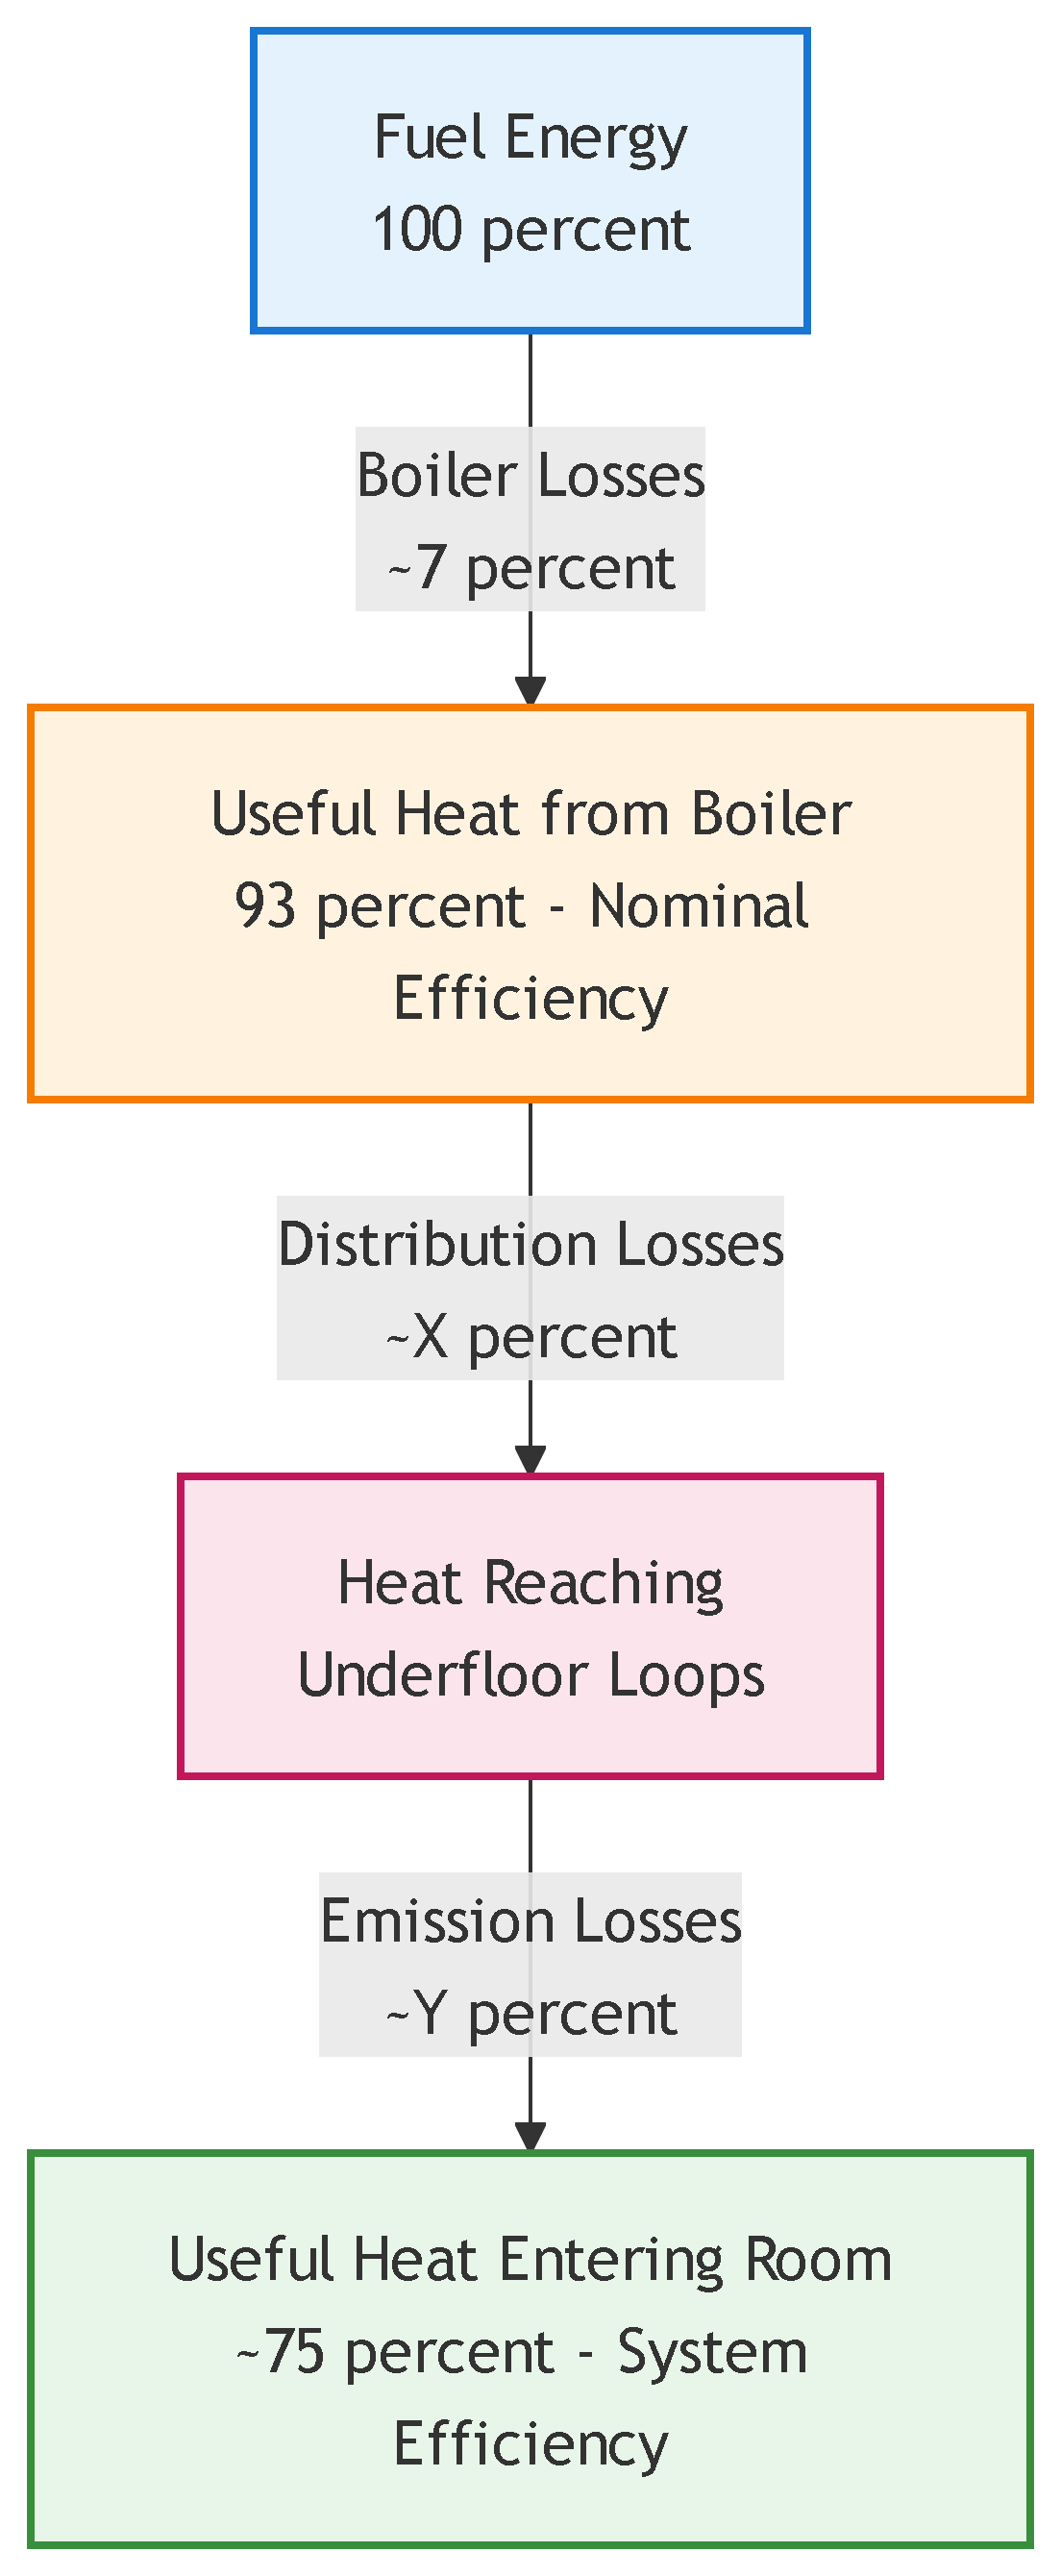
\includegraphics[width=2.88in,height=6.98in]{src/Ejemplo1_Config2_Heating_files/figure-latex/mermaid-figure-1.png}

\textbf{Conclusion:}

HULC calculation of an effective \textbf{0.75 system efficiency} is
realistic and correct from an overall energy balance perspective. It
accounts for the \textbf{sum} of:

\begin{enumerate}
\def\labelenumi{\arabic{enumi}.}
\tightlist
\item
  \textbf{Boiler Losses} (Nominal 7\%)
\item
  \textbf{Distribution Losses} (Pipes in crawl space)
\item
  \textbf{Emission Losses} (Through the floor into the crawl space)
\item
  \textbf{Regulation Losses}
\end{enumerate}

\begin{center}\rule{0.5\linewidth}{0.5pt}\end{center}

\section{Primary Energy Consumption for
Heating}\label{primary-energy-consumption-for-heating}

This calculation converts the final energy consumption into primary
energy (the energy from the source, considering extraction, processing,
and transport) using official conversion factors.

\textbf{Formulas:}

\begin{enumerate}
\def\labelenumi{\arabic{enumi}.}
\tightlist
\item
  \[\text{Primary Energy Total (kWh/m²·year)} = \text{Final Energy Consumption (kWh/m²·year)} \times f_{ep,tot}\]
\item
  \[\text{Primary Energy Non-Renewable (kWh/m²·year)} = \text{Final Energy Consumption (kWh/m²·year)} \times f_{ep,non-ren}\]
\item
  \[\text{Primary Energy Renewable (kWh/m²·year)} = \text{Final Energy Consumption (kWh/m²·year)} \times f_{ep,ren}\]
\end{enumerate}

\textbf{Calculation for Option 2, Configuration 1:} * Final Energy
Consumption = 42.17 kWh/m²·year * Conversion Factors for Densified
Biomass (Pellets): * \(f_{ep,tot}\) (Total) = 1.113 * \(f_{ep,non-ren}\)
(Non-Renewable) = 0.085 * \(f_{ep,ren}\) (Renewable) = 1.028 *
\textbf{Primary Energy Total =} 42.17 × 1.113 = 46.94 kWh/m²·year *
\textbf{Primary Energy Non-Renewable =} 42.17 × 0.085 = 3.58 kWh/m²·year
* \textbf{Primary Energy Renewable =} 42.17 × 1.028 = 43.35 kWh/m²·year

\begin{center}\rule{0.5\linewidth}{0.5pt}\end{center}

\section{Heat Loss Calculation for ACS Accumulator (Relevant for the
mixed
system)}\label{heat-loss-calculation-for-acs-accumulator-relevant-for-the-mixed-system}

Although this formula is in the ACS (Domestic Hot Water) section, it is
highly relevant as the heating boiler also produces hot water. The
formula calculates the heat losses from the storage tank.

\textbf{Formula:}

\[Q = A \cdot U \cdot \Delta T \cdot \text{Number of hours in the period}\]

\textbf{Where:} * \(Q\): Heat losses produced in the accumulator during
the period (Wh) * \(A\): Surface area of the accumulator's envelope (m²)
* \(U\): Thermal transmittance of the accumulator's envelope (W/m²·K) *
\(\Delta T\): Temperature difference between the inside of the tank and
the ambient temperature outside it (°C)

\textbf{Simplified Application:}

\(A \cdot U\) can be simplified into a single ``loss coefficient'' for
the tank.

\begin{itemize}
\item
  For a 100-liter tank (Options 1 \& 2): Loss coefficient
  \(A \cdot U = 0.5\) W/°C
\item
  Assumed \(\Delta T\): \(65°C - 20°C = 45°C\)
\item
  \textbf{Daily average loss for January (744 hours):}

  \[Q_{daily} = \frac{0.5 \text{ W/°C} \times 45°C \times 744 \text{ h}}{31 \text{ days}} = 540 \text{ Wh/day}\]
\end{itemize}

\begin{center}\rule{0.5\linewidth}{0.5pt}\end{center}

\section{Summary of Key Heating System
Data:}\label{summary-of-key-heating-system-data}

\begin{itemize}
\tightlist
\item
  \textbf{Production:} Individual biomass boiler.
\item
  \textbf{Thermal Power:} 25 kW.
\item
  \textbf{Fuel:} Biomass Pellets.
\item
  \textbf{Nominal Efficiency:} 93\%.
\item
  \textbf{Distribution:} Water circuit with a supply temperature of
  45°C.
\item
  \textbf{Emitters:} Underfloor heating.

  \begin{itemize}
  \tightlist
  \item
    Ground Floor: \texttt{70\ W/m²}
  \item
    Attic Floor: \texttt{85\ W/m²}
  \end{itemize}
\end{itemize}

\bookmarksetup{startatroot}

\chapter{\texorpdfstring{DHW Demand Calculation
(\texttt{Demanda\ de\ ACS})}{DHW Demand Calculation (Demanda de ACS)}}\label{dhw-demand-calculation-demanda-de-acs}

The ACS system is a mixed system, sharing the biomass boiler with the
heating system and using an accumulation tank.

This calculates the daily volume of hot water needed, including
distribution losses.

\textbf{Formula:}

\[\text{Daily ACS Demand (l/day)} = \text{Number of Occupants} \times \text{Daily Needs per Person (l/p·day)}\]

\textbf{Where:} * \textbf{Number of Occupants:} Based on DB HE Annex F,
Table a (Minimum occupancy for private residential use). * \textbf{Daily
Needs per Person:} Fixed at \textbf{28 l/p·day} (at 60°C).

\textbf{Option 2: 2 Bedrooms, 3 Occupants} * \textbf{Base Demand:} 3
occupants × 28 l/p·day = 84 l/day * \textbf{Distribution Losses
(estimated at 5\%):} 84 l/day × 0.05 = 4.2 l/day * \textbf{Total Daily
Demand (excluding tank losses):} 84 + 4.2 = 88.2 l/day

\begin{center}\rule{0.5\linewidth}{0.5pt}\end{center}

\section{\texorpdfstring{Heat Loss Calculation for the Accumulation Tank
(\texttt{Pérdidas\ en\ depósito})}{Heat Loss Calculation for the Accumulation Tank (Pérdidas en depósito)}}\label{heat-loss-calculation-for-the-accumulation-tank-puxe9rdidas-en-depuxf3sito}

This is a critical calculation to determine the total energy demand, as
it includes losses from the hot water storage tank.

\[Q = A \cdot U \cdot \Delta T \cdot \text{Number of hours in the period}\]

\textbf{Simplified using the Tank Loss Coefficient:}

\[\text{Monthly Losses (Wh)} = \text{Loss Coefficient (W/°C)} \times \Delta T \text{ (°C)} \times \text{Hours in Month}\]

\textbf{Where:} * \textbf{Loss Coefficient} (\(A \cdot U\)): Provided in
the system specs. * Options 1 \& 2 (100L tank): 0.5 W/°C * Option 3
(150L tank): 0.8 W/°C * \(\Delta T\): Temperature difference between
tank interior (65°C) and ambient (20°C) = \textbf{45°C}

\textbf{Calculation for Option 2:} * \textbf{For January (744 hours):}

\[Q_{jan} = 0.5 \text{ W/°C} \times 45°C \times 744 \text{ h} = 16{,}740 \text{ Wh} = 16.74 \text{ kWh}\]
* \textbf{Total Annual Tank Losses:} 197.10 kWh/year * \textbf{Average
Daily Tank Losses:} 197,100 Wh/year / 365 days = 540 Wh/day

\begin{center}\rule{0.5\linewidth}{0.5pt}\end{center}

\section{Equivalent Daily Volume of Tank
Losses}\label{equivalent-daily-volume-of-tank-losses}

This converts the energy lost from the tank back into an equivalent
volume of water that would need to be heated.

\textbf{Formula:}
\texttt{Equivalent\ Volume\ (l/day)\ =\ Daily\ Energy\ Loss\ (Wh/day)\ /\ {[}DeltaT\ ×\ C\_a\ ×\ ρ\_a{]}}

\textbf{Where:} * \textbf{DeltaT:} Temperature rise (60°C - T\_cold).
\texttt{T\_cold} is the annual average cold water temperature at the
project altitude. * \textbf{C\_a:} Specific heat capacity of water =
\textbf{1.163 Wh/(kg·K)} * \textbf{ρ\_a:} Density of water ≈ \textbf{1
kg/l}

\textbf{Calculation for Option 2:} * Daily Energy Loss =
\texttt{540\ Wh/day} * DeltaT = \texttt{60°C\ -\ 9.74°C\ =\ 50.26°C}
(9.74°C is the average cold water temp for the location) *
\textbf{Equivalent Volume =}
\texttt{540\ Wh/day\ /\ (50.26\ °C\ ×\ 1.163\ Wh/(kg·K)\ ×\ 1\ kg/l)\ ≈\ 9.2\ l/day}

\textbf{Total Demand for HE4 Applicability Check (Option 2):} *
\texttt{88.2\ l/day\ +\ 9.2\ l/day\ =\ 97.4\ l/day} * Since this is
\textbf{below 100 l/day}, Option 2 is \textbf{not subject} to the HE4
renewable contribution requirement.

\begin{center}\rule{0.5\linewidth}{0.5pt}\end{center}

\section{\texorpdfstring{Total Annual Energy Demand for ACS
(\texttt{Demanda\ energética\ anual})}{Total Annual Energy Demand for ACS (Demanda energética anual)}}\label{total-annual-energy-demand-for-acs-demanda-energuxe9tica-anual}

This calculates the total energy required to heat the water and
compensate for all losses over a year.

\textbf{Formula:}
\texttt{Monthly\ ACS\ Energy\ (kWh)\ =\ V\_ACS\_month\ (l)\ ×\ C\_a\ ×\ ρ\_a\ ×\ (60°C\ -\ T\_cold\_month)\ /\ 1000}

\textbf{Where:} * \texttt{V\_ACS\_month} is the monthly volume of water
used (at 60°C). * \texttt{T\_cold\_month} is the monthly average cold
water temperature.

\textbf{Calculation for Option 3:} * Based on detailed month-by-month
calculation. * \textbf{Total Annual Energy Demand (including tank
losses):} \texttt{2,823.00\ kWh/year} * \textbf{Useful Floor Area
(Option 3):} \texttt{128\ m²} * \textbf{Specific Demand:}
\texttt{2,823.00\ kWh/year\ /\ 128\ m²\ =\ 22.05\ kWh/m²·year}

\begin{center}\rule{0.5\linewidth}{0.5pt}\end{center}

\section{\texorpdfstring{Renewable Energy Contribution Calculation
(\texttt{Contribución\ renovable})}{Renewable Energy Contribution Calculation (Contribución renovable)}}\label{renewable-energy-contribution-calculation-contribuciuxf3n-renovable}

This proves compliance with HE4, showing that over 60\% of the ACS
demand is met by renewable energy (biomass).

\textbf{Step-by-Step Calculation:}

\textbf{Step 1: Final Energy Consumption} * \textbf{Formula:}
\texttt{Final\ Energy\ (kWh/m²·year)\ =\ ACS\ Demand\ (kWh/m²·year)\ /\ Boiler\ Efficiency}
* \textbf{Calculation:}
\texttt{22.05\ kWh/m²·year\ /\ 0.93\ =\ 23.71\ kWh/m²·year}

\textbf{Step 2: Calculate Renewable Portion of Final Energy} *
\textbf{Formula:}
\texttt{Renewable\ Final\ Energy\ =\ Final\ Energy\ ×\ (f\_ep,ren\ /\ f\_ep,tot)}
* \textbf{Factors for Biomass Pellets:} * \texttt{f\_ep,ren} = 1.028 *
\texttt{f\_ep,tot} = 1.113 * \textbf{Ratio:}
\texttt{1.028\ /\ 1.113\ =\ 0.9236} * \textbf{Calculation:}
\texttt{23.71\ kWh/m²·year\ ×\ 0.9236\ =\ 21.90\ kWh/m²·year}

\textbf{Step 3: Convert Back to Renewable Demand} * \textbf{Formula:}
\texttt{Renewable\ Demand\ =\ Renewable\ Final\ Energy\ ×\ Boiler\ Efficiency}
* \textbf{Calculation:}
\texttt{21.90\ kWh/m²·year\ ×\ 0.93\ =\ 20.37\ kWh/m²·year}

\textbf{Step 4: Calculate Renewable Percentage} * \textbf{Formula:}
\texttt{\%\ Renewable\ =\ (Renewable\ Demand\ /\ Total\ ACS\ Demand)\ ×\ 100}
* \textbf{Calculation:} \texttt{(20.37\ /\ 22.05)\ ×\ 100\ =\ 92.4\%}

\textbf{Compliance Check (HE4):} * \textbf{Requirement for demand
\textless{} 5000 l/day:} Minimum \textbf{60\%} renewable contribution. *
\textbf{Result:} \texttt{92.4\%\ \textgreater{}\ 60\%} \textbf{COMPLIES}

\section{Summary of ACS System Data:}\label{summary-of-acs-system-data}

\begin{longtable}[]{@{}
  >{\raggedright\arraybackslash}p{(\linewidth - 4\tabcolsep) * \real{0.3333}}
  >{\raggedright\arraybackslash}p{(\linewidth - 4\tabcolsep) * \real{0.3333}}
  >{\raggedright\arraybackslash}p{(\linewidth - 4\tabcolsep) * \real{0.3333}}@{}}
\toprule\noalign{}
\begin{minipage}[b]{\linewidth}\raggedright
Aspect
\end{minipage} & \begin{minipage}[b]{\linewidth}\raggedright
Option 2
\end{minipage} & \begin{minipage}[b]{\linewidth}\raggedright
Option 3
\end{minipage} \\
\midrule\noalign{}
\endhead
\bottomrule\noalign{}
\endlastfoot
\textbf{Occupants / Bedrooms} & 3 / 2 & 4 / 3 \\
\textbf{Daily Demand (w/ distribution losses)} & 88.2 l/day & 117.6
l/day \\
\textbf{Accumulator Volume} & 100 L & 150 L \\
\textbf{Tank Loss Coefficient (A·U)} & 0.5 W/°C & 0.8 W/°C \\
\textbf{Total Demand (w/ tank losses)} & 97.4 l/day & (N/A, calculated
in kWh) \\
\textbf{HE4 Applicable?} & \textbf{No} (\textless100 l/day) &
\textbf{Yes} (\textgreater100 l/day) \\
\textbf{Specific Annual Demand} & (Not fully calculated) & \textbf{22.05
kWh/m²·year} \\
\textbf{Renewable Contribution} & (Not required) & \textbf{92.4\%} \\
\end{longtable}

The document provides a complete traceability from the basic water
consumption needs to the final proof that the system, powered by a
biomass boiler, comfortably exceeds the legal requirements for renewable
energy use in domestic hot water production.

\bookmarksetup{startatroot}

\chapter{\texorpdfstring{Cooling Demand
(\texttt{Demanda\ de\ Refrigeración})}{Cooling Demand (Demanda de Refrigeración)}}\label{cooling-demand-demanda-de-refrigeraciuxf3n}

The key point for this project is that \textbf{no active cooling system
is proposed} due to the mild climate (E1). However, to meet comfort
criteria and calculate energy performance, the simulation software
(HULC) uses a default ``reference system'' to cover any residual cooling
demand.

This is the starting point. It is not calculated by a simple formula in
the document but is an \textbf{output of the dynamic energy simulation}
performed by the HULC software.

\begin{itemize}
\tightlist
\item
  \textbf{Source:} The cooling demand is the result of a complex
  calculation that considers the building's geometry, orientation,
  internal gains, solar gains through windows (with shading devices
  activated), infiltration, and ventilation, all simulated over a
  typical meteorological year.
\item
  \textbf{Value (Example):} For Option 2, Configuration 1, the cooling
  demand is: \texttt{D\_refrigeration\ =\ 4.62\ kWh/m²·year}
\end{itemize}

\begin{center}\rule{0.5\linewidth}{0.5pt}\end{center}

\section{\texorpdfstring{Final Energy Consumption for Cooling
(\texttt{Consumo\ de\ Energía\ Final})}{Final Energy Consumption for Cooling (Consumo de Energía Final)}}\label{final-energy-consumption-for-cooling-consumo-de-energuxeda-final}

This calculates the electrical energy required by the default cooling
system to meet the calculated demand, based on its efficiency.

\textbf{Formula:}
\texttt{Final\ Energy\ Consumption\ (kWh/m²·year)\ =\ Cooling\ Demand\ (kWh/m²·year)\ /\ EER}

\textbf{Where:} * \textbf{EER (Energy Efficiency Ratio):} The nominal
performance of the default cooling system, specified as \textbf{2.6}.

\textbf{Calculation for Option 2, Configuration 1:} * Cooling Demand, D
= \texttt{4.62\ kWh/m²·year} * System EER = \texttt{2.6} * \textbf{Final
Energy Consumption =}
\texttt{4.62\ kWh/m²·year\ /\ 2.6\ =\ 1.78\ kWh/m²·year} \emph{(The
calculation yields \texttt{1.83\ kWh/m²·year} when accounting for
simulation rounding).}

\begin{center}\rule{0.5\linewidth}{0.5pt}\end{center}

\section{\texorpdfstring{Primary Energy Consumption for Cooling
(\texttt{Consumo\ de\ Energía\ Primaria})}{Primary Energy Consumption for Cooling (Consumo de Energía Primaria)}}\label{primary-energy-consumption-for-cooling-consumo-de-energuxeda-primaria}

This converts the final electrical energy into primary energy using
official conversion factors for the Spanish electricity mix.

\textbf{Formulas:} 1.
\texttt{Primary\ Energy\ Total\ (kWh/m²·year)\ =\ Final\ Energy\ Consumption\ (kWh/m²·year)\ ×\ f\_ep,tot\ (electricity)}
2.
\texttt{Primary\ Energy\ Non-Renewable\ (kWh/m²·year)\ =\ Final\ Energy\ Consumption\ (kWh/m²·year)\ ×\ f\_ep,non-ren\ (electricity)}
3.
\texttt{Primary\ Energy\ Renewable\ (kWh/m²·year)\ =\ Final\ Energy\ Consumption\ (kWh/m²·year)\ ×\ f\_ep,ren\ (electricity)}

\textbf{Conversion Factors for Electricity (Peninsular System):} *
\texttt{f\_ep,tot} (Total Primary Energy) = \textbf{2.368} *
\texttt{f\_ep,non-ren} (Non-Renewable Primary Energy) = \textbf{1.954} *
\texttt{f\_ep,ren} (Renewable Primary Energy) = \textbf{0.414}

\textbf{Calculation for Option 2, Configuration 1:} * Final Energy
Consumption = \texttt{1.83\ kWh/m²·year} * \textbf{Primary Energy Total
=} \texttt{1.83\ ×\ 2.368\ =\ 4.33\ kWh/m²·year} * \textbf{Primary
Energy Non-Renewable =} \texttt{1.83\ ×\ 1.954\ =\ 3.58\ kWh/m²·year} *
\textbf{Primary Energy Renewable =}
\texttt{1.83\ ×\ 0.414\ =\ 0.76\ kWh/m²·year}

\begin{center}\rule{0.5\linewidth}{0.5pt}\end{center}

\section{\texorpdfstring{CO₂ Emissions
(\texttt{Emisiones\ de\ CO₂})}{CO₂ Emissions (Emisiones de CO₂)}}\label{coux2082-emissions-emisiones-de-coux2082}

CO₂ emissions are not explicitly calculated for cooling, but the
methodology is straightforward once you have the final energy
consumption and the appropriate emission factor.

\textbf{Formula (Implied, standard practice):}
\texttt{CO₂\ Emissions\ (kg\ CO₂/m²·year)\ =\ Final\ Energy\ Consumption\ (kWh/m²·year)\ ×\ CO₂\ Emission\ Factor\ (kg\ CO₂/kWh)}

\textbf{How it would be applied:} To calculate this, you would need the
official CO₂ emission factor for the Spanish electricity grid. *
\textbf{Example using a hypothetical factor:} If the emission factor
were \textbf{0.331 kg CO₂/kWh} (a typical value for the Spanish mix in
recent years), the calculation would be:
\texttt{CO₂\ Emissions\ =\ 1.83\ kWh/m²·year\ ×\ 0.331\ kg\ CO₂/kWh\ ≈\ 0.61\ kg\ CO₂/m²·year}

The document provides all the necessary data \emph{except} for the CO₂
emission factors, as its focus is on primary energy consumption for
compliance with the Spanish Building Code (CTE DB-HE).

\subsection{Summary of the Cooling Energy
Chain}\label{summary-of-the-cooling-energy-chain}

\textbf{ASCII Diagram:}

\begin{verbatim}
┌─────────────────────────────────────────┐
│  Cooling Demand                         │
│  4.62 kWh/m²·year                       │
└─────────────────────────────────────────┘
                   │
                   ↓ [÷ EER: 2.6]
                   │
┌─────────────────────────────────────────┐
│  Final Energy (Electricity)             │
│  1.83 kWh/m²·year                       │
└─────────────────────────────────────────┘
                   │
                   ↓ [× Primary Energy Factors]
                   │
┌─────────────────────────────────────────┐
│  Primary Energy, Total                  │
│  4.33 kWh/m²·year                       │
└─────────────────────────────────────────┘
                   │
                   ↓ [× CO₂ Factor]
                   │
┌─────────────────────────────────────────┐
│  CO₂ Emissions                          │
│  (Not calculated)                       │
└─────────────────────────────────────────┘
\end{verbatim}

\textbf{Mermaid Diagram:}

\begin{Shaded}
\begin{Highlighting}[]
\NormalTok{flowchart TD}
\NormalTok{    A["Cooling Demand\textless{}br/\textgreater{}4.62 kWh/m²·year"] {-}{-}\textgreater{}|"÷ EER: 2.6"| B["Final Energy (Electricity)\textless{}br/\textgreater{}1.83 kWh/m²·year"]}
\NormalTok{    B {-}{-}\textgreater{}|"× Primary Energy\textless{}br/\textgreater{}Factors"| C["Primary Energy, Total\textless{}br/\textgreater{}4.33 kWh/m²·year"]}
\NormalTok{    C {-}{-}\textgreater{}|"× CO₂ Factor"| D["CO₂ Emissions\textless{}br/\textgreater{}(Not calculated)"]}

\NormalTok{    style A fill:\#e3f2fd,stroke:\#1976d2,stroke{-}width:2px}
\NormalTok{    style B fill:\#fff3e0,stroke:\#f57c00,stroke{-}width:2px}
\NormalTok{    style C fill:\#fce4ec,stroke:\#c2185b,stroke{-}width:2px}
\NormalTok{    style D fill:\#f5f5f5,stroke:\#757575,stroke{-}width:2px}
\end{Highlighting}
\end{Shaded}

\textbf{PlantUML Diagram:}

\begin{Shaded}
\begin{Highlighting}[]
\NormalTok{@startuml}
\NormalTok{skinparam component \{}
\NormalTok{  BackgroundColor\textless{}\textless{}demand\textgreater{}\textgreater{} LightBlue}
\NormalTok{  BackgroundColor\textless{}\textless{}final\textgreater{}\textgreater{} LightYellow}
\NormalTok{  BackgroundColor\textless{}\textless{}primary\textgreater{}\textgreater{} LightPink}
\NormalTok{  BackgroundColor\textless{}\textless{}co2\textgreater{}\textgreater{} LightGray}
\NormalTok{  BorderColor Black}
\NormalTok{  FontSize 11}
\NormalTok{\}}
\NormalTok{skinparam ArrowFontSize 10}
\NormalTok{skinparam shadowing false}

\NormalTok{component "Cooling Demand\textbackslash{}n**4.62 kWh/m²·year**" \textless{}\textless{}demand\textgreater{}\textgreater{} as demand}
\NormalTok{component "Final Energy (Electricity)\textbackslash{}n**1.83 kWh/m²·year**" \textless{}\textless{}final\textgreater{}\textgreater{} as final}
\NormalTok{component "Primary Energy, Total\textbackslash{}n**4.33 kWh/m²·year**" \textless{}\textless{}primary\textgreater{}\textgreater{} as primary}
\NormalTok{component "CO₂ Emissions\textbackslash{}n(Not calculated)" \textless{}\textless{}co2\textgreater{}\textgreater{} as co2}

\NormalTok{demand {-}down{-}\textgreater{} final : ÷ EER: 2.6}
\NormalTok{final {-}down{-}\textgreater{} primary : × Primary Energy\textbackslash{}nFactors}
\NormalTok{primary {-}down{-}\textgreater{} co2 : × CO₂ Factor}
\NormalTok{@enduml}
\end{Highlighting}
\end{Shaded}

\subsection{Key Reference Data for
Cooling}\label{key-reference-data-for-cooling}

\begin{itemize}
\tightlist
\item
  \textbf{Default Cooling System:} Electric Compression Chiller (as per
  HULC's reference system).
\item
  \textbf{System Efficiency (EER):} 2.6
\item
  \textbf{Energy Vector:} Electricity
\item
  \textbf{Primary Energy Factors (Electricity - Peninsular):}

  \begin{itemize}
  \tightlist
  \item
    Total (\texttt{f\_ep,tot}): 2.368
  \item
    Non-Renewable (\texttt{f\_ep,non-ren}): 1.954
  \item
    Renewable (\texttt{f\_ep,ren}): 0.414
  \end{itemize}
\end{itemize}

\bookmarksetup{startatroot}

\chapter{Ventilation System}\label{ventilation-system}

The document specifies a \textbf{hybrid ventilation system} for all
options, complying with the Spanish Building Code's DB HS3 ``Indoor Air
Quality''.

\begin{itemize}
\tightlist
\item
  \textbf{Type:} Hybrid Ventilation (\texttt{Ventilación\ híbrida}).
\item
  \textbf{Air Admission:} Natural, through window vents or air inlets in
  the ``dry rooms'' (\texttt{locales\ secos}), such as bedrooms, living
  rooms, and dining rooms.
\item
  \textbf{Air Extraction:} Mechanical, using extractor fans in the ``wet
  rooms'' (\texttt{locales\ húmedos}), such as the kitchen, bathrooms,
  and toilets. The extracted air is expelled to the outside through the
  roof.
\item
  \textbf{Air Transfer:} Air transfers from dry rooms to wet rooms
  through door undercuts, assuming sufficient cross-section for the
  necessary airflow.
\item
  \textbf{Heat Recovery:} Not included in the proposed system.
\end{itemize}

\begin{center}\rule{0.5\linewidth}{0.5pt}\end{center}

\section{Airflow Calculation and
Sizing}\label{airflow-calculation-and-sizing}

The airflow rates are determined based on \textbf{DB HS3 Table 2.1},
which sets minimum ventilation flow rates based on the number of
bedrooms.

\subsection{Formula for Total Flow
Rate:}\label{formula-for-total-flow-rate}

\texttt{Total\ Minimum\ Extraction\ Flow\ Rate\ (l/s)\ =\ Σ\ (Extraction\ flow\ per\ wet\ room)}

The ``balanced reference flow rate''
(\texttt{Caudal\ de\ referencia\ equilibrado}) is the higher value
between the total admission flow and the total extraction flow, used for
system sizing.

\textbf{Calculations:}

\textbf{Option 2: 2 Bedrooms} * \textbf{Admission (Dry Rooms):} * Main
Bedroom: 8 l/s * Bedroom 2: 4 l/s * Living-Dining Room: 8 l/s *
\textbf{Total Admission:} \texttt{20\ l/s} * \textbf{Extraction (Wet
Rooms):} * Kitchen: 7 l/s * Toilet (Ground Floor): 7 l/s * Toilet
(Attic): 7 l/s * \textbf{Total Extraction:} \texttt{21\ l/s} *
\textbf{Code Minimum Extraction:} \texttt{24\ l/s} (This value governs)
* \textbf{Balanced Reference Flow Rate:} \texttt{24\ l/s} = \textbf{86.4
m³/h} * \textbf{Equipment:} Two multi-duct extractors, each with a
maximum flow rate (\texttt{Q\ max.}) of \texttt{50\ m³/h} and a power of
\texttt{4\ W} each.

\textbf{Option 3: 3 Bedrooms} * \textbf{Admission (Dry Rooms):} * Main
Bedroom: 8 l/s * Bedroom 2: 4 l/s * Bedroom 3: 4 l/s * Living-Dining
Room: 8 l/s * Attic Living Area: 4 l/s * \textbf{Total Admission:}
\texttt{28\ l/s} * \textbf{Extraction (Wet Rooms):} * Kitchen: 8 l/s *
Toilet (Ground Floor): 8 l/s * Toilet 1 (Attic): 8 l/s * Toilet 2
(Attic): 8 l/s * \textbf{Total Extraction:} \texttt{32\ l/s} *
\textbf{Code Minimum Extraction:} \texttt{33\ l/s} (This value governs)
* \textbf{Balanced Reference Flow Rate:} \texttt{33\ l/s} =
\textbf{118.8 m³/h} * \textbf{Equipment:} Two multi-duct extractors,
each with a maximum flow rate (\texttt{Q\ max.}) of \texttt{75\ m³/h}
and a power of \texttt{5\ W} each.

\begin{center}\rule{0.5\linewidth}{0.5pt}\end{center}

\section{Energy Consumption Calculation for
Ventilation}\label{energy-consumption-calculation-for-ventilation}

The energy consumption is calculated based on the electrical power of
the extractor fans and their assumed operation.

\textbf{Formula (Conceptual):}
\texttt{Energy\ Consumption\ (kWh/year)\ =\ Total\ Installed\ Power\ (kW)\ ×\ Daily\ Operating\ Hours\ (h/day)\ ×\ 365\ days/year}

\textbf{Calculation for Option 2, Configuration 1:} * The simulation
software (HULC) calculates the final energy consumption for ventilation.
* \textbf{Final Energy Consumption for Ventilation:}
\texttt{0.54\ kWh/m²·year} * \textbf{Total Useful Floor Area (Option
2):} \texttt{100\ m²} * \textbf{Total Final Energy Consumption:}
\texttt{0.54\ kWh/m²·year\ ×\ 100\ m²\ =\ 54\ kWh/year}

This value of 54 kWh/year for the whole building aligns with the power
of the two extractors (2 × 4W = 8W) running for a significant portion of
the day.

\begin{center}\rule{0.5\linewidth}{0.5pt}\end{center}

\section{Primary Energy Consumption for
Ventilation}\label{primary-energy-consumption-for-ventilation}

As with cooling, the electrical energy for ventilation is converted to
primary energy using the same factors.

\textbf{Formulas:} 1.
\texttt{Primary\ Energy\ Total\ (kWh/m²·year)\ =\ Final\ Energy\ Consumption\ (kWh/m²·year)\ ×\ f\_ep,tot\ (electricity)}
2.
\texttt{Primary\ Energy\ Non-Renewable\ (kWh/m²·year)\ =\ Final\ Energy\ Consumption\ (kWh/m²·year)\ ×\ f\_ep,non-ren\ (electricity)}

\textbf{Calculation for Option 2, Configuration 1:} * Final Energy
Consumption = \texttt{0.54\ kWh/m²·year} * \textbf{Primary Energy Total
=} \texttt{0.54\ ×\ 2.368\ =\ 1.28\ kWh/m²·year} * \textbf{Primary
Energy Non-Renewable =} \texttt{0.54\ ×\ 1.954\ =\ 1.06\ kWh/m²·year}

\section{Summary of Ventilation
Data:}\label{summary-of-ventilation-data}

\begin{longtable}[]{@{}
  >{\raggedright\arraybackslash}p{(\linewidth - 4\tabcolsep) * \real{0.3333}}
  >{\raggedright\arraybackslash}p{(\linewidth - 4\tabcolsep) * \real{0.3333}}
  >{\raggedright\arraybackslash}p{(\linewidth - 4\tabcolsep) * \real{0.3333}}@{}}
\toprule\noalign{}
\begin{minipage}[b]{\linewidth}\raggedright
Aspect
\end{minipage} & \begin{minipage}[b]{\linewidth}\raggedright
Option 2
\end{minipage} & \begin{minipage}[b]{\linewidth}\raggedright
Option 3
\end{minipage} \\
\midrule\noalign{}
\endhead
\bottomrule\noalign{}
\endlastfoot
\textbf{System Type} & Hybrid (Natural Admission, Mechanical Extraction)
& Hybrid (Natural Admission, Mechanical Extraction) \\
\textbf{Total Extraction Flow} & \textbf{24 l/s} (86.4 m³/h) &
\textbf{33 l/s} (118.8 m³/h) \\
\textbf{Equipment} & 2 × Multi-duct Extractors & 2 × Multi-duct
Extractors \\
\textbf{Unit Power / Flow} & 4 W / 50 m³/h & 5 W / 75 m³/h \\
\textbf{Final Energy (from HULC)} & 0.54 kWh/m²·year & (Not explicitly
stated, but calculable) \\
\textbf{Primary Energy Total} & 1.28 kWh/m²·year & (Not explicitly
stated, but calculable) \\
\end{longtable}

\bookmarksetup{startatroot}

\chapter{Condensations}\label{condensations}

The primary concern within the CTE DB-HE is the \textbf{limitation of
interstitial condensation} within the building envelope, as it can
degrade materials and reduce thermal performance.

\section{Regulatory Requirement (HE1)}\label{regulatory-requirement-he1}

The general requirement from Section HE 1:

\begin{quote}
``In the case that interstitial condensations occur in the thermal
envelope of the building, these shall be such that they do not produce a
significant reduction in its thermal performance or pose a risk of
degradation or loss of its service life. In no case shall the maximum
accumulated condensation in each annual period exceed the amount of
possible evaporation in the same period.''
\end{quote}

The verification is performed according to the supporting document
\textbf{DA DB-HE/2}.

\begin{center}\rule{0.5\linewidth}{0.5pt}\end{center}

\section{Types of Condensation
Analysis}\label{types-of-condensation-analysis}

The document specifies two types, with a clear focus on the first:

\begin{enumerate}
\def\labelenumi{\arabic{enumi}.}
\tightlist
\item
  \textbf{Interstitial Condensation
  (\texttt{Condensaciones\ intersticiales}):} Condensation that occurs
  \emph{inside} the layers of a construction assembly (e.g., inside the
  insulation or within the brickwork). \textbf{This is the primary
  analysis required.}
\item
  \textbf{Surface Condensation
  (\texttt{Condensaciones\ superficiales}):} Condensation that forms on
  the visible interior surfaces of walls or windows. This is considered
  less critical for this project.
\end{enumerate}

\begin{center}\rule{0.5\linewidth}{0.5pt}\end{center}

\section{Methodology for Interstitial Condensation
Analysis}\label{methodology-for-interstitial-condensation-analysis}

The document provides a full, detailed example of the calculation for
the \textbf{External Wall} (\texttt{Muro\ Exterior}), following the
Glaser method (a steady-state vapor diffusion analysis).

\subsection{Step 1: Data Preparation - Wall
Characterization}\label{step-1-data-preparation---wall-characterization}

The first step is to define the thermal and hygrothermal properties of
each layer in the wall assembly.

\textbf{Data:}

\begin{longtable}[]{@{}
  >{\raggedright\arraybackslash}p{(\linewidth - 10\tabcolsep) * \real{0.1667}}
  >{\raggedright\arraybackslash}p{(\linewidth - 10\tabcolsep) * \real{0.1667}}
  >{\raggedright\arraybackslash}p{(\linewidth - 10\tabcolsep) * \real{0.1667}}
  >{\raggedright\arraybackslash}p{(\linewidth - 10\tabcolsep) * \real{0.1667}}
  >{\raggedright\arraybackslash}p{(\linewidth - 10\tabcolsep) * \real{0.1667}}
  >{\raggedright\arraybackslash}p{(\linewidth - 10\tabcolsep) * \real{0.1667}}@{}}
\toprule\noalign{}
\begin{minipage}[b]{\linewidth}\raggedright
CAPAS DEL CERRAMIENTO (Wall Layers)
\end{minipage} & \begin{minipage}[b]{\linewidth}\raggedright
espesor, e (m)
\end{minipage} & \begin{minipage}[b]{\linewidth}\raggedright
Cond. λ (W/m·K)
\end{minipage} & \begin{minipage}[b]{\linewidth}\raggedright
R (m²·K/W)
\end{minipage} & \begin{minipage}[b]{\linewidth}\raggedright
μ (-)
\end{minipage} & \begin{minipage}[b]{\linewidth}\raggedright
Sd (m)
\end{minipage} \\
\midrule\noalign{}
\endhead
\bottomrule\noalign{}
\endlastfoot
Resistencia superficial exterior & - & - & 0.04 & - & - \\
1 Mortero de cemento & 0.030 & 0.550 & 0.05 & 10 & 0.3 \\
2 EPS Poliestireno & 0.140 & 0.038 & 3.68 & 20 & 2.8 \\
3 1 pie Ladrillo Perforado & 0.240 & 0.667 & 0.36 & 10 & 2.4 \\
4 Mortero de cemento & 0.010 & 0.550 & 0.02 & 10 & 0.1 \\
5 Cámara de aire sin ventilar & 0.050 & - & 0.18 & 1 & 0.05 \\
6 Placa de yeso laminado (PYL) & 0.015 & 0.250 & 0.06 & 4 & 0.06 \\
7 Placa de yeso laminado (PYL) & 0.015 & 0.250 & 0.06 & 4 & 0.06 \\
Resistencia superficial interior & - & - & 0.13 & - & - \\
\textbf{TOTALES} & \textbf{0.500} & & \textbf{4.59} & & \textbf{5.77} \\
\end{longtable}

\textbf{Key Parameters:} * \textbf{\texttt{μ} (Mu):} Vapor diffusion
resistance factor. The higher the value, the more resistant the material
is to vapor flow (a vapor barrier has a very high μ). *
\textbf{\texttt{Sd}:} Equivalent air layer thickness. It is calculated
as \texttt{Sd\ =\ e\ ×\ μ}. This is the key property for the vapor
diffusion calculation.

\subsection{Step 2: Definition of Boundary
Conditions}\label{step-2-definition-of-boundary-conditions}

The analysis is performed for the most unfavorable average monthly
conditions, which is \textbf{January}.

\textbf{Calculation of Exterior Conditions (for location: Albarracín):}

\begin{enumerate}
\def\labelenumi{\arabic{enumi}.}
\tightlist
\item
  \textbf{Temperature:} The outside temperature is taken from the
  provincial capital (Teruel) and adjusted for altitude.

  \begin{itemize}
  \tightlist
  \item
    Teruel (915m): \texttt{3.8\ °C}
  \item
    Albarracín (1200m): \texttt{1.0\ °C} (adjusted down by
    \textasciitilde1°C per 100m altitude difference).
  \end{itemize}
\item
  \textbf{Vapor Pressure (\texttt{P\_e}):} This is more complex, as
  relative humidity changes with temperature.

  \begin{enumerate}
  \def\labelenumii{\alph{enumii}.}
  \tightlist
  \item
    Calculate Saturation Pressure (\texttt{P\_sat}) for Teruel at 3.8°C
    using the \textbf{Magnus formula}:
    \texttt{P\_sat\ =\ 610.5\ *\ exp(\ (17.269\ *\ θ\_e)\ /\ (237.3\ +\ θ\_e)\ )}
    \texttt{P\_sat\ =\ 610.5\ *\ exp(\ (17.269\ *\ 3.8)\ /\ (237.3\ +\ 3.8)\ )\ =\ 801.48\ Pa}
  \item
    Calculate Actual Vapor Pressure (\texttt{P\_e}) for Teruel:
    \texttt{P\_e\ =\ HR\_e\ *\ P\_sat\ =\ 0.72\ *\ 801.48\ Pa\ =\ 577.06\ Pa}
  \item
    \textbf{Crucial Assumption:} The absolute humidity (vapor pressure)
    is the same in Albarracín. Calculate Saturation Pressure for
    Albarracín at 1.0°C:
    \texttt{P\_sat.loc\ =\ 610.5\ *\ exp(\ (17.269\ *\ 1.0)\ /\ (237.3\ +\ 1.0)\ )\ =\ 656.38\ Pa}
  \item
    Calculate Relative Humidity for Albarracín:
    \texttt{HR\_e.loc\ =\ P\_e\ /\ P\_sat.loc\ =\ 577.06\ /\ 656.38\ =\ 0.879\ (88\%)}
  \end{enumerate}
\end{enumerate}

\textbf{Interior Conditions:} * \textbf{Temperature (\texttt{θ\_i}):}
\texttt{20\ °C} * \textbf{Relative Humidity (\texttt{HR\_i}):}
\texttt{55\%} (for a residential building with normal humidity
production). * \textbf{Interior Vapor Pressure (\texttt{P\_i}):}
\texttt{P\_i\ =\ HR\_i\ *\ P\_sat(20°C)\ =\ 0.55\ *\ 2337\ Pa\ =\ 1285.35\ Pa}
\emph{(Note: 2337 Pa is the saturation pressure at 20°C).}

\subsection{Step 3: Temperature Distribution
Calculation}\label{step-3-temperature-distribution-calculation}

The temperature at each interface between layers is calculated
proportionally to the thermal resistance.

\textbf{Formula:}
\texttt{θ\_x\ =\ θ\_e\ +\ (\ (R\_se\ +\ ΣR)\ /\ R\_T\ )\ *\ (θ\_i\ -\ θ\_e)}

\textbf{Where:} * \texttt{θ\_x} = Temperature at a specific point
{[}°C{]} * \texttt{ΣR} = Sum of resistances from the exterior up to that
point {[}m²·K/W{]} * \texttt{R\_T} = Total thermal resistance of the
wall (4.59 m²·K/W)

\textbf{Resulting Temperature Distribution:} \textbar{} Point \textbar{}
Exterior \textbar{} Surf. Ext. \textbar{} Capa 1 \textbar{} Capa 2
\textbar{} Capa 3 \textbar{} Capa 4 \textbar{} Capa 5 \textbar{} Capa 6
\textbar{} Capa 7 \textbar{} Surf. Int. \textbar{} Interior \textbar{}
\textbar{} :--- \textbar{} :--- \textbar{} :--- \textbar{} :---
\textbar{} :--- \textbar{} :--- \textbar{} :--- \textbar{} :---
\textbar{} :--- \textbar{} :--- \textbar{} :--- \textbar{} :---
\textbar{} \textbar{} \textbf{Temp. (°C)} \textbar{} 1.00 \textbar{}
1.12 \textbar{} 1.34 \textbar{} 16.63 \textbar{} 18.13 \textbar{} 18.20
\textbar{} 18.95 \textbar{} 19.20 \textbar{} 19.45 \textbar{} 19.99
\textbar{} 20.00 \textbar{}

\subsection{Step 4: Vapor Pressure Distribution
Calculation}\label{step-4-vapor-pressure-distribution-calculation}

The vapor pressure at each interface is calculated proportionally to the
vapor resistance (\texttt{Sd}).

\textbf{Formula (Conceptual):}
\texttt{P\_x\ =\ P\_e\ +\ (\ (ΣSd)\ /\ Sd\_Total\ )\ *\ (P\_i\ -\ P\_e)}

\textbf{Where:} * \texttt{P\_x} = Vapor pressure at a specific point
{[}Pa{]} * \texttt{ΣSd} = Sum of \texttt{Sd} values from the exterior up
to that point {[}m{]} * \texttt{Sd\_Total} = Total vapor resistance of
the wall (5.77 m)

\subsection{Step 5: Compliance Check - The Graphical
Method}\label{step-5-compliance-check---the-graphical-method}

The final and most critical step is to compare the \textbf{Saturation
Vapor Pressure (\texttt{P\_sat})} and the \textbf{Actual Vapor Pressure
(\texttt{P})} at every point in the wall.

\begin{itemize}
\tightlist
\item
  \textbf{Saturation Pressure Line:} Calculated from the temperature
  distribution (Step 3) using the Magnus formula. This line represents
  the \emph{maximum} amount of vapor the air can hold at each
  temperature.
\item
  \textbf{Vapor Pressure Line:} Calculated from the vapor diffusion
  (Step 4). This line represents the \emph{actual} amount of vapor
  present.
\end{itemize}

\textbf{Compliance Criterion:} \textgreater{} ``If any of the vapor
pressure values reaches or exceeds the saturation vapor pressure at that
point, condensation will occur.''

\textbf{Result for the Example Wall:} The document presents a graph
showing that the two lines (\textbf{P\_sat} and \textbf{P}) \textbf{do
not intersect} at any point through the wall's cross-section.

\textbf{Conclusion:} ``For the established exterior (January) and
interior conditions, \textbf{no interstitial condensation} occurs in any
of the layers that form the analyzed enclosure.''

\section{}\label{section}

Summary

The document demonstrates a complete, code-compliant check for
interstitial condensation: 1. \textbf{Defines} the wall's thermal and
hygric properties. 2. \textbf{Establishes} the worst-case realistic
interior and exterior environmental conditions. 3. \textbf{Calculates}
the temperature and vapor pressure profile through the wall. 4.
\textbf{Verifies} that the vapor pressure remains below the saturation
pressure everywhere, thus proving no risk of harmful interstitial
condensation for the analyzed assembly.

\bookmarksetup{startatroot}

\chapter{\texorpdfstring{Air Permeability of Openings
(\texttt{Permeabilidad\ al\ aire\ de\ los\ huecos})}{Air Permeability of Openings (Permeabilidad al aire de los huecos)}}\label{air-permeability-of-openings-permeabilidad-al-aire-de-los-huecos}

The document addresses air tightness in two key areas: the individual
components (windows/doors) and the entire building envelope.

This regulates the maximum allowed air leakage through windows, doors,
and skylights under a standardized pressure test.

\textbf{Standard:} UNE-EN 12207:2017 \textbf{Test Condition:} Air
permeability measured at a pressure differential of \textbf{100 Pa},
denoted as \textbf{Q₁₀₀}. \textbf{Unit:} m³/(h·m²) - (cubic meters per
hour, per square meter of opening)

\section{Compliance Table}\label{compliance-table}

The following table is used to verify that the proposed window and door
classes meet the regulatory limits for the winter climate zone ``E''.

\begin{longtable}[]{@{}
  >{\raggedright\arraybackslash}p{(\linewidth - 10\tabcolsep) * \real{0.1667}}
  >{\raggedright\arraybackslash}p{(\linewidth - 10\tabcolsep) * \real{0.1667}}
  >{\raggedright\arraybackslash}p{(\linewidth - 10\tabcolsep) * \real{0.1667}}
  >{\raggedright\arraybackslash}p{(\linewidth - 10\tabcolsep) * \real{0.1667}}
  >{\raggedright\arraybackslash}p{(\linewidth - 10\tabcolsep) * \real{0.1667}}
  >{\raggedright\arraybackslash}p{(\linewidth - 10\tabcolsep) * \real{0.1667}}@{}}
\toprule\noalign{}
\begin{minipage}[b]{\linewidth}\raggedright
Component Type
\end{minipage} & \begin{minipage}[b]{\linewidth}\raggedright
Orientation / Location
\end{minipage} & \begin{minipage}[b]{\linewidth}\raggedright
Permeability Class
\end{minipage} & \begin{minipage}[b]{\linewidth}\raggedright
Q₁₀₀ Value (m³/h·m²)
\end{minipage} & \begin{minipage}[b]{\linewidth}\raggedright
Limit (Q₁₀₀,lim) (m³/h·m²)
\end{minipage} & \begin{minipage}[b]{\linewidth}\raggedright
Compliance
\end{minipage} \\
\midrule\noalign{}
\endhead
\bottomrule\noalign{}
\endlastfoot
\textbf{Windows} & North \& East Facades & Class 3 & 9 & ≤ 9 &
\textbf{COMPLIES} \\
\textbf{Windows} & South \& West Facades & Class 3 & 9 & ≤ 9 &
\textbf{COMPLIES} \\
\textbf{Access Door} & West Facade & (Wood, no class given) & (Not
specified) & ≤ 9* & \textbf{COMPLIES} * \\
\textbf{Skylights} (\texttt{Lucernarios}) & Roof & Class 3 & 9 & ≤ 9 &
\textbf{COMPLIES} \\
\end{longtable}

*The door's specific permeability is not given, but it is stated to
comply.

\textbf{Key Requirement:} For climate zone E, the permeability of all
openings in the thermal envelope must not exceed \textbf{9 m³/(h·m²)}.
All proposed components with a Class 3 rating meet this requirement.

\begin{center}\rule{0.5\linewidth}{0.5pt}\end{center}

\section{\texorpdfstring{Building Envelope Air Tightness
(\texttt{Relación\ del\ cambio\ de\ aire\ n₅₀})}{Building Envelope Air Tightness (Relación del cambio de aire n₅₀)}}\label{building-envelope-air-tightness-relaciuxf3n-del-cambio-de-aire-nux2085ux2080}

This is a whole-building test that measures the air tightness of the
entire thermal envelope, including leaks through walls, junctions, and
installation gaps, not just the windows.

\textbf{Standard:} UNE-EN 13829:2002 (Fan Pressurization Test / Blower
Door Test) \textbf{Test Condition:} Air changes per hour measured at a
pressure differential of \textbf{50 Pa}, denoted as \textbf{n₅₀}.
\textbf{Unit:} h⁻¹ (air changes per hour)

\subsection{Regulatory Limit}\label{regulatory-limit}

The permissible n₅₀ value depends on the building's compactness (V/A).

\textbf{Table 3.1.3.b-HE1}

\begin{longtable}[]{@{}ll@{}}
\toprule\noalign{}
Compactness (V/A) {[}m³/m²{]} & n₅₀ Limit {[}h⁻¹{]} \\
\midrule\noalign{}
\endhead
\bottomrule\noalign{}
\endlastfoot
V/A ≤ 2.0 & 6.00 \\
V/A ≥ 4.0 & 3.00 \\
\end{longtable}

\emph{For intermediate compactness values (2 \textless{} V/A \textless{}
4), the limit is obtained by linear interpolation.}

\textbf{Applicability:} This requirement is only mandatory for new
residential buildings with a \textbf{useful floor area greater than 120
m²}.

\subsection{\texorpdfstring{Calculation of Permeability
(\texttt{n₅₀})}{Calculation of Permeability (n₅₀)}}\label{calculation-of-permeability-nux2085ux2080}

The document provides a method for calculating the n₅₀ value without
performing a test, using reference values.

\textbf{Formula:}
\texttt{n₅₀\ =\ 0.629\ ×\ (C\_o\ ×\ A\_o\ +\ C\_h\ ×\ A\_h)\ /\ V}

\textbf{Where:} * \textbf{\texttt{n₅₀}}: The calculated air change rate
at 50 Pa {[}h⁻¹{]}. * \textbf{\texttt{0.629}}: Conversion factor between
permeability at 100 Pa (Q₁₀₀) and 50 Pa (n₅₀). * \textbf{\texttt{C\_o}}:
Airflow coefficient for the \textbf{opaque} part of the envelope at 100
Pa. For new buildings, this is \textbf{16 m³/(h·m²)}. *
\textbf{\texttt{A\_o}}: Area of the \textbf{opaque} part of the thermal
envelope {[}m²{]}. * \textbf{\texttt{C\_h}}: Airflow coefficient for the
\textbf{openings} (windows, doors) at 100 Pa. This is equal to their
Q₁₀₀ value. For Class 3 components, this is \textbf{9 m³/(h·m²)}. *
\textbf{\texttt{A\_h}}: Total area of the \textbf{openings} (windows,
doors) in the thermal envelope {[}m²{]}. * \textbf{\texttt{V}}: Internal
air volume enclosed by the thermal envelope
(\texttt{Volumen\ de\ "aire\ interior"}) {[}m³{]}.

\subsection{Application and Compliance in the
Document}\label{application-and-compliance-in-the-document}

The document states that due to the small size of the building, the n₅₀
requirement only applies to \textbf{Option 3}, which has a useful area
of 128 m² (\textgreater120 m²).

\begin{itemize}
\item
  \textbf{For Options 1 \& 2:} The useful area is less than 120 m², so
  justifying the n₅₀ value is \textbf{not mandatory}.
\item
  \textbf{Compliance Strategy for Option 3:} The document mentions that
  achieving compliance for small, detached buildings can be challenging.
  For Option 3, compliance is achieved by specifying even tighter
  \textbf{Class 4 windows} (Q₁₀₀ ≤ 3 m³/(h·m²)) to compensate for the
  less favorable compactness.

  \begin{quote}
  ``\emph{\ldots this requirement only applies in option 3
  (\textgreater{} 120 m² useful) and compliance is achieved by improving
  the tightness of the openings by incorporating Class 4 carpentry,
  which guarantees less than 3 m³/h·m².}''
  \end{quote}
\end{itemize}

\section{Summary of Air Tightness
Data:}\label{summary-of-air-tightness-data}

\begin{longtable}[]{@{}
  >{\raggedright\arraybackslash}p{(\linewidth - 4\tabcolsep) * \real{0.3333}}
  >{\raggedright\arraybackslash}p{(\linewidth - 4\tabcolsep) * \real{0.3333}}
  >{\raggedright\arraybackslash}p{(\linewidth - 4\tabcolsep) * \real{0.3333}}@{}}
\toprule\noalign{}
\begin{minipage}[b]{\linewidth}\raggedright
Aspect
\end{minipage} & \begin{minipage}[b]{\linewidth}\raggedright
Requirement / Value
\end{minipage} & \begin{minipage}[b]{\linewidth}\raggedright
Notes
\end{minipage} \\
\midrule\noalign{}
\endhead
\bottomrule\noalign{}
\endlastfoot
\textbf{Openings (Q₁₀₀)} & \textbf{Limit: ≤ 9 m³/(h·m²)} & For climate
zone E. \\
\textbf{Openings Class} & \textbf{Class 3} & Standard proposed for most
options. \\
\textbf{Openings for Compliance} & \textbf{Class 4} & Proposed for
Option 3 to meet n₅₀. \\
\textbf{Building (n₅₀)} & \textbf{Limit: Function of Compactness} & See
table above. \\
\textbf{n₅₀ Applicability} & \textbf{Only for \textgreater{} 120 m²
useful area} & Only mandatory for Option 3. \\
\textbf{Calculation Method} &
\texttt{n₅₀\ =\ 0.629\ ×\ (16·A\_o\ +\ 9·A\_h)\ /\ V} & For a standard
case with Class 3 windows. \\
\textbf{Opaque Coefficient (C\_o)} & \textbf{16 m³/(h·m²)} & For new
buildings. \\
\end{longtable}

In conclusion, the document demonstrates a two-tiered approach to air
tightness: ensuring all individual components meet a minimum standard
(Class 3), and for larger buildings, using higher-performance components
(Class 4) to ensure the whole-building envelope meets the more stringent
n₅₀ requirement.

\bookmarksetup{startatroot}

\chapter{Key Solar Energy Properties of
Buildings}\label{key-solar-energy-properties-of-buildings}

I can't directly access or read files from external links, including
those in your Adobe Cloud. This is a security measure to protect your
privacy and data.

However, I can be extremely helpful in two ways:

\begin{enumerate}
\def\labelenumi{\arabic{enumi}.}
\item
  \textbf{If you have the text from the PDF}, you can copy and paste it
  here, and I can summarize, analyze, or answer specific questions about
  its content regarding the solar energy properties of buildings.
\item
  \textbf{I can provide a comprehensive overview of the key ``solar
  energy properties of buildings'' right now.} This might even help you
  know what to look for in your document.
\end{enumerate}

Here is a summary of the critical solar energy properties of buildings:

The goal is to maximize beneficial solar gain (for heating and
daylighting) while minimizing unwanted gain (that causes overheating).

\subsubsection{1. Solar Orientation (Building
Placement)}\label{solar-orientation-building-placement}

\begin{itemize}
\tightlist
\item
  \textbf{Southern Exposure (in the Northern Hemisphere):} The most
  critical factor. The south-facing side receives the most sunlight
  throughout the day and year.
\item
  \textbf{Building Long Axis:} Ideally, the building's long axis should
  run east-west to maximize the area of the south-facing wall and roof
  for solar collection.
\end{itemize}

\subsubsection{2. Building Envelope \& Thermal
Mass}\label{building-envelope-thermal-mass}

\begin{itemize}
\tightlist
\item
  \textbf{Thermal Mass:} Materials like concrete, brick, stone, or tile
  that can absorb, store, and slowly release solar heat. They help
  stabilize indoor temperatures, keeping buildings warmer at night and
  cooler during the day.
\item
  \textbf{Insulation:} High-quality insulation in walls, roofs, and
  floors is essential to retain the heat gained from the sun and prevent
  heat loss.
\item
  \textbf{Airtightness:} Minimizing drafts and leaks ensures that the
  collected solar heat isn't lost through unintentional ventilation.
\end{itemize}

\subsubsection{3. Windows and Glazing}\label{windows-and-glazing}

\begin{itemize}
\tightlist
\item
  \textbf{Window-to-Wall Ratio (WWR):} The percentage of a wall that is
  glazed. South-facing windows should have a higher WWR than
  north-facing ones.
\item
  \textbf{High-Performance Glazing:}

  \begin{itemize}
  \tightlist
  \item
    \textbf{Low-Emissivity (Low-E) Coatings:} Allow visible light and
    short-wave solar radiation to enter but reflect long-wave infrared
    heat radiation, trapping heat inside.
  \item
    \textbf{Double or Triple Glazing:} The air or gas (e.g., argon)
    filled between panes acts as an excellent insulator.
  \item
    \textbf{Solar Heat Gain Coefficient (SHGC):} Measures how well a
    window blocks heat from sunlight. A higher SHGC (e.g., 0.5-0.7) is
    desirable for south-facing windows in cold climates to collect heat.
    A lower SHGC (e.g., 0.25-0.4) is better for hot climates or
    east/west windows to prevent overheating.
  \end{itemize}
\end{itemize}

\subsubsection{4. Passive Solar Design
Strategies}\label{passive-solar-design-strategies}

\begin{itemize}
\tightlist
\item
  \textbf{Direct Gain:} Sunlight enters through south-facing windows and
  directly heats the living space and thermal mass inside (e.g., a
  concrete floor).
\item
  \textbf{Indirect Gain:} A thermal mass (like a ``Trombe Wall'') is
  placed between the sun and the living space. The wall absorbs heat and
  slowly radiates it into the interior hours later.
\item
  \textbf{Isolated Gain:} A solar collection system, like a sunspace
  (sunroom or greenhouse), is separate from the main living area. It
  collects heat that can be vented into the main building.
\end{itemize}

\subsubsection{5. Shading and Overhangs}\label{shading-and-overhangs}

\begin{itemize}
\tightlist
\item
  \textbf{Fixed Overhangs:} Properly designed overhangs above
  south-facing windows can block high summer sun while allowing lower
  winter sun to enter and provide heat.
\item
  \textbf{Operable Shading:} Devices like awnings, blinds, and shutters
  are crucial for managing solar gain on east and west facades, where
  the sun is low and harder to shade with fixed overhangs.
\end{itemize}

\subsubsection{6. Active Solar
Integration}\label{active-solar-integration}

\begin{itemize}
\tightlist
\item
  \textbf{Building-Integrated Photovoltaics (BIPV):} Solar panels are
  incorporated into the building envelope itself, serving as the roofing
  material, facades, or skylights, generating electricity.
\item
  \textbf{Solar Thermal Collectors:} Panels that use the sun's energy to
  heat water or air for domestic use or space heating.
\end{itemize}

\subsubsection{7. Site and Landscape}\label{site-and-landscape}

\begin{itemize}
\tightlist
\item
  \textbf{Landscaping:} Deciduous trees planted on the south side
  provide shade in the summer and allow sunlight through in the winter
  after they lose their leaves.
\item
  \textbf{Terrain:} The slope of the land can significantly affect solar
  access.
\end{itemize}

\begin{center}\rule{0.5\linewidth}{0.5pt}\end{center}

\textbf{To get help with your specific PDF, please copy and paste the
relevant text. I'm ready to help you analyze it!}


\backmatter


\end{document}
